\documentclass[tikz,border=6pt]{standalone}
\usepackage{amsmath,amssymb}
\usepackage{xcolor}
\definecolor{accent}{HTML}{A13D2C}
\definecolor{accent2}{HTML}{2B5F6B}
\definecolor{muted}{HTML}{5A564F}
\definecolor{linecol}{HTML}{D8D2C4}
\definecolor{astroblue}{HTML}{1B4F72}
\definecolor{sunyellow}{HTML}{E8A33D}
\usetikzlibrary{calc,arrows.meta}
\begin{document}
% Model rotation curve (all analytic, G = 4.301e-6 kpc (km/s)^2 / Msun).
% Stars: enclosed mass M r^2/(r+a)^2, M = 6e10 Msun, a = 1.5 kpc  ->  v^2 = 258060 r/(r+1.5)^2.
% Halo: rho = rho_c/(1+r^2/r_c^2), r_c = 4 kpc, 4 pi G rho_c r_c^2 = (200 km/s)^2
%   -> v^2 = 200^2 [1 - (r_c/r) atan(r/r_c)];  for r < 2 kpc the series u^2/3 - u^4/5 + u^6/7 - u^8/9, u = r/4.
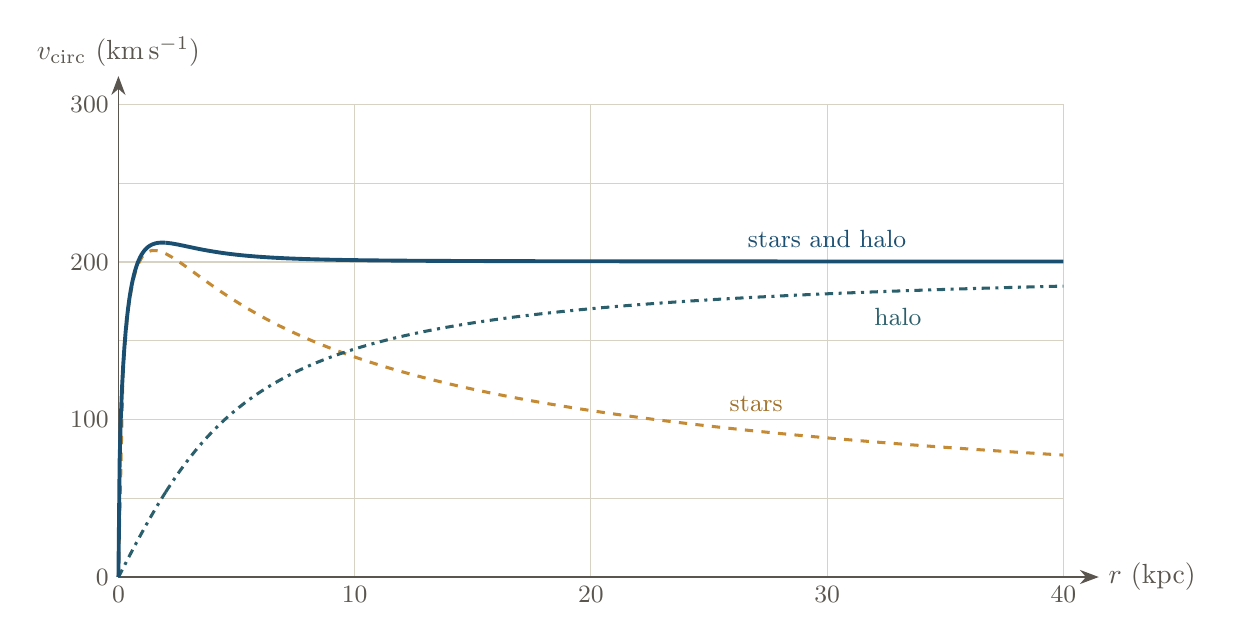
\begin{tikzpicture}[x=0.3cm,y=0.02cm, >={Stealth[length=2.4mm]}]
  \foreach \y in {50,100,...,300} \draw[linecol] (0,\y) -- (40,\y);
  \foreach \x in {10,20,30,40} \draw[linecol] (\x,0) -- (\x,300);
  \draw[->, muted] (0,0) -- (41.5,0) node[right] {$r$ (kpc)};
  \draw[->, muted] (0,0) -- (0,318) node[above] {$v_{\rm circ}$ (km\,s$^{-1}$)};
  \foreach \x in {0,10,20,30,40} \node[below, muted] at (\x,0) {\small \x};
  \foreach \y in {0,100,200,300} \node[left, muted] at (0,\y) {\small \y};
  % stars alone
  \draw[sunyellow!85!black, line width=1.1pt, dashed, domain=0:40, samples=200]
    plot (\x, {100*sqrt(25.806*\x/((\x+1.5)*(\x+1.5)))});
  % halo alone
  \draw[accent2, line width=1.1pt, dash dot, domain=0:2, samples=30]
    plot (\x, {200*sqrt((\x/4)^2/3 - (\x/4)^4/5 + (\x/4)^6/7 - (\x/4)^8/9)});
  \draw[accent2, line width=1.1pt, dash dot, domain=2:40, samples=150]
    plot (\x, {200*sqrt(1 - (4/\x)*rad(atan(\x/4)))});
  % total: v^2 adds
  \draw[astroblue, line width=1.4pt, domain=0:2, samples=40]
    plot (\x, {100*sqrt(25.806*\x/((\x+1.5)*(\x+1.5)) + 4*((\x/4)^2/3 - (\x/4)^4/5 + (\x/4)^6/7 - (\x/4)^8/9))});
  \draw[astroblue, line width=1.4pt, domain=2:40, samples=150]
    plot (\x, {100*sqrt(25.806*\x/((\x+1.5)*(\x+1.5)) + 4*(1 - (4/\x)*rad(atan(\x/4))))});
  \node[astroblue, above] at (30,203) {\small stars and halo};
  \node[accent2] at (33,165) {\small halo};
  \node[sunyellow!70!black] at (27,110) {\small stars};
\end{tikzpicture}
\end{document}
